%!TEX program = xelatex
\documentclass[12pt]{article}
\usepackage[top=1.5cm, left=2cm, right=2cm, bottom=1.5cm]{geometry} % Symmetrical margins
\usepackage{graphicx}
\usepackage{amsmath}
\usepackage{fontspec}
\usepackage{polyglossia}
% \usepackage[polutonikogreek,english]{hyphenat}
\usepackage{xunicode}
\usepackage{xltxtra}
\usepackage{float}
\usepackage{placeins}
\usepackage{indentfirst}
\usepackage{nicefrac}
\usepackage{booktabs}
\usepackage{array}
\usepackage{xcolor}
\usepackage{minted}
\usepackage{varwidth}

\usepackage[
    backend=biber,
    sorting=nyt
]{biblatex}
\addbibresource{references.bib}
\DefineBibliographyStrings{greek}{
    andothers = {κ.α}
}
\DeclareFieldFormat*{title}{\textnormal{#1}}
%\usepackage[utf8]{inputenc}
%\usepackage[greek,english]{babel}
\setdefaultlanguage[variant=monotonic]{greek}
\setotherlanguage{english}

\usepackage[colorlinks=true,
            linkcolor=blue,
            urlcolor=blue,
            citecolor=blue]{hyperref}

\setmainfont[Scale=1.09]{DejaVuSans}
\newfontfamily\greekfont[Scale=1.09]{FreeSerif}
\newfontfamily\greekfontsf[Scale=1.09]{FreeSans}
\newfontfamily\greekfonttt[Scale=1.09]{FreeMono}
\setromanfont{FreeSerif}
\setsansfont{FreeSans}
\setmonofont{FreeMono}

\setminted{fontsize=\small}
\usemintedstyle{perldoc}
% \definecolor{monokai}{RGB}{39,40,34}
\definecolor{paraiso-light}{RGB}{231, 233, 219}


\usepackage{titlesec}

\titleformat{\section}
    {\normalfont\Large\bfseries}
    {\thesection}
    {1.5em}
    {\vspace{1em}}
%\setlength{\droptitle}{-3cm}

\begin{document}

\title{Crimmins Speckle Removal Filter}
\author{Αναστάσιος Φραγκόπουλος 58633}
\date{}


\begin{titlepage}
    \begin{center}
        \vspace*{1.5cm}

        \textbf{\LARGE Crimmins Speckle Removal Filter}

        \vspace{0.5cm}
        {\large Τεχνολογία Παράλληλης Επεξεργασίας}

        \vspace{1.5cm}

        \textbf{Αναστάσιος Φραγκόπουλος 58633}

        \vfill

        Πρώτη εξαμηνιαία εργασία

        Ακαδ. Έτος 2024-2025

        \vspace{0.8cm}

        Εργαστήριο Αρχιτεκτονικής Υπολογιστών και Συστημάτων Υψηλών Επιδόσεων\\
        Δημοκρίτειο Πανεπιστήμιο Θράκης\\
        Τμήμα Ηλεκτρολόγων Μηχανικών και Μηχανικών Υπολογιστών\\

    \end{center}
\end{titlepage}


\section{Σειριακός Αλγόριθμος}

Ο Crimmins Speckle removal είναι ένας αλγόριθμος που μειώνει από ασπρόμαυρες εικόνες τον θόρυβο salt-and-pepper, που είναι ένα είδος θορύβου που δίνει την εμφάνιση μίας εικόνας πασπαλισμένης με αλάτι και πιπέρι. Οι επανειλημμένες χρήσεις του αλγόριθμου σε μια εικόνα δίνουν καλύτερα αποτελέσματα μείωσης του θορύβου αλλά προκαλούν θόλωση της εικόνας.

Ο αλγόριθμος αρχικά αυξάνει την φωτεινότητα των pixel που είναι σκοτεινότερα από τους γείτονες του και μετά μειώνοντας την φωτεινότητα των pixel που είναι φωτεινότερα από τους γείτονες του. Η σύγκρηση αυτή γίνεται μεταξύ του κάθε pixel και ζευγαριού pixel των 8 γειτόνων για μια κατεύθυνση σε κάθε πέρασμα (πάνω-κάτω, δεξιά-αριστερά, διαγώνια αριστερά-δεξιά, διαγώνια δεξιά-αριστερά).

Για κάθε επανάληψη του αλγορίθμου, γίνονται πρώτα οι παρακάτω συγκρίσεις για την διόρθωσή των σκοτεινών pixel για τις τέσσερεις κατευθύνσεις

\begin{minted}[breaklines, breaksymbolright={}, breaksymbolleft={}, bgcolor=paraiso-light]{c}
    uint8_t dark_pass_logic(uint8_t a, uint8_t b, uint8_t c)
    {
            if(a >= b + 2) b++;
            if(a > b && b <= c) b++;
            if(c > b && b <= a) b++;
            if(c >= b + 2) b++;
            return b;
    }
\end{minted}

και έπειτα οι παρακάτω συγκρίσεις για την διόρθωση των φωτεινών pixel για τις τέσσερεις κατευθύνσεις

\begin{minted}[breaklines, breaksymbolright={}, breaksymbolleft={}, bgcolor=paraiso-light]{c}
    uint8_t light_pass_logic(uint8_t a, uint8_t b, uint8_t c)
    {
            if(a <= b - 2) b--;
            if(a < b && b >= c) b--;
            if(c < b && b >= a) b--;
            if(c <= b - 2) b--;
            return b;
    }
\end{minted}

Όπου b το κεντρικό pixel κάθε γειτονιάς και a, c το ζευγάρι pixel για μια κατεύθυνσή (π.χ. για την επανάληψη πάνω-κάτω το a θα είναι το pixel πάνω από το b και το c το pixel κάτω από το b).\\

Οπότε για μία επανάληψη του, ο αλγόριθμος περνάει όλα τα pixel μίας εικόνας τέσσερις φορές για την διόρθωση των σκοτεινών και άλλες τέσσερεις για την διόρθωση των φωτεινών pixel. Δηλαδή κάνει $8\cdot m \cdot n$ επαναλήψεις όπου m το πλάτος και n το μήκος της εικόνας σε pixel. Άρα η πολυπλοκότητα του είναι  $\mathrm{O}(k \cdot m \cdot n)$, όπου k είναι ο αριθμός των επαναλήψεων του αλγόριθμου για μια εικόνα.

\begin{figure}[H]
    \centering
    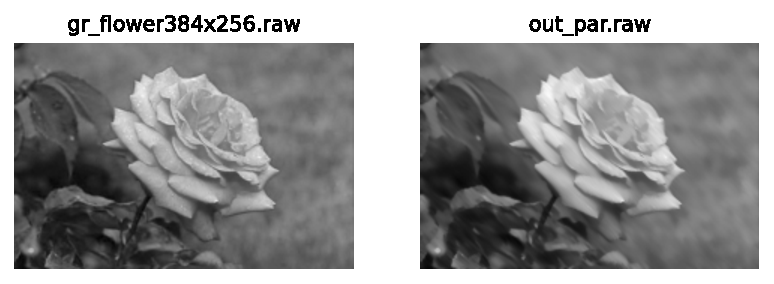
\includegraphics[width=0.8\linewidth]{./pics/gr_flower384x256.pdf}
    \caption{Παράδειγμα αλγορίθμου για 2 επαναλήψεις}
\end{figure}

\begin{figure}[H]
    \centering
    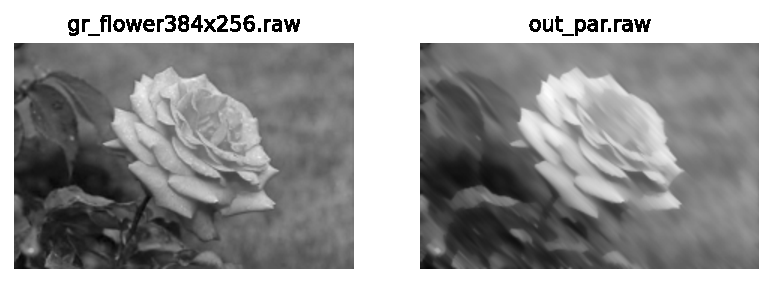
\includegraphics[width=0.8\linewidth]{./pics/gr_flower384x256_blur.pdf}
    \caption{Παράδειγμα αλγορίθμου για 8 επαναλήψεις}
\end{figure}

\vspace{2em}

\section{Υλοποίηση του αλγόριθμου}

Κύριο στοιχείο στην υλοποίηση του αλγόριθμου είναι η συνάρτηση που είναι υπεύθυνη για το πέρασμα του κάθε pixel της εικόνας και είναι φτιαγμένη έτσι ώστε να μπορεί να ξαναχρησιμοποιηθεί για όλες τις κατευθύνσεις ανάλογα με την είσοδο που της δίνεται. Επιπλέον, οι συναρτήσεις που κάνουν την σύγκρισή των γειτονικών pixel, που αναφέρθηκαν παραπάνω δίνονται ως είσοδος στην συνάρτηση για τον ίδιο λόγο. Η κάθε επανάληψη της εξωτερικής for loop μεταβάλει την γραμμή της εικόνας στην οποία βρισκόμαστε και η εσωτερική μεταβάλει την στήλη της εικόνας στην οποία βρισκόμαστε. Στην αλλαγή γραμμής υπολογίζουμε έναν pointer που δείχνει στην αρχή κάθε γραμμής, για το a, b, c, ώστε να γλιτώσουμε ένα μέρος των πράξεων που χρειάζεται στις επαναλήψεις του άξονα x. Τέλος, γράφει στο pixel b την τιμή διασφαλίζοντας ότι θα είναι μεταξύ 0 και 255.

\newpage

\begin{minted}[breaklines, breaksymbolright={}, breaksymbolleft={}, bgcolor=paraiso-light]{c}
void pass_func(uint8_t *image, uint8_t *tmp_image, uint32_t width,
    uint32_t height, int dx, int dy,
    uint8_t (*pass_logic_func)(uint8_t, uint8_t, uint8_t)) {

    for(int y = 1; y < height - 1; y++) {
        uint8_t *row_a = tmp_image + (y-dy) * width;
        uint8_t *row_b = tmp_image + y * width;
        uint8_t *row_c = tmp_image + (y+dy) * width;
        uint8_t *row_out = image + y * width;

        for(int x = 1; x < width - 1; x++) {
            uint8_t a = row_a[x-dx];
            uint8_t b = row_b[x];
            uint8_t c = row_c[x+dx];

            b = pass_logic_func(a, b, c);
            row_out[x] = (b < 0) ? 0 : (b > 255) ? 255 : b;
        }
    }
}
\end{minted}

Οι πράξεις για την επιλογή των a, b, c φαίνεται από το παρακάτω διάγραμμα που δείχνει τις συντεταγμένες (x, y) του κάθε pixel μίας γειτονιάς.

\vspace{0.3em}
\begin{center}
\begin{varwidth}{0.6\linewidth}
\begin{minted}[breaklines, breaksymbolright={}, breaksymbolleft={}, bgcolor=paraiso-light]{sh}
 +------------+------------+------------+ 
 |            |            |            | 
 |  y-1, x-1  |   y-1, x   |  y-1, x+1  | 
 |            |            |            | 
 +------------+------------+------------+ 
 |            |            |            | 
 |  y,   x-1  |   y,   x   |  y,   x+1  | 
 |            |            |            | 
 +------------+------------+------------+ 
 |            |            |            | 
 |  y+1, x-1  |   y+1, x   |  y+1, x+1  | 
 |            |            |            | 
 +------------+------------+------------+ 
\end{minted}
\end{varwidth}
\end{center}

Όπως φαίνεται από την συνάρτηση για κάθε μία από τις 8 επανάληψης της πρέπει να της δίνουμε δύο εικόνες, μία με την προηγούμενη κατάσταση της εικόνας και μία στην οποία θα γράψουμε το αποτέλεσμα. Για να αποφύγουμε την συνεχείς δημιουργία και διαγραφή των buffer μεταξύ των επαναλήψεων, επέλεξα να ανταλλάσω τους pointer των εικόνων, έτσι ώστε η εικόνα στην οποία γράφεται το αποτέλεσμα στην επόμενη επανάληψη να γίνεται η προηγούμενη κατάσταση και η προηγούμενη κατάσταση να γίνεται το καινούργιο αποτέλεσμα.

\newpage

\section{Παράλληλη υλοποίηση του Αλγόριθμου}

Στον Crimmins Speckle removal αλγόριθμο το μόνο που πρέπει να παραμένει σειριακό είναι η σειρά με την οποία κάνουμε τα περάσματα για την διόρθωση των pixel για κάθε κατεύθυνση. Για τον λόγο αυτό επέλεξα να παραλληλοποιήσω την συνάρτηση που είναι υπεύθυνη για αυτά τα περάσματα. Έκανα την εξωτερική for loop παράλληλη έτσι ώστε να χωριστεί η εικόνα σε $\nicefrac{\Large n}{\Large p}$ κομμάτια όπου n οι γραμμές της εικόνας και p οι πυρήνες του συστήματος.

\begin{minted}[breaklines, breaksymbolright={}, breaksymbolleft={}, bgcolor=paraiso-light]{c}
void pass_func_par(uint8_t *image, uint8_t *tmp_image, uint32_t width,
    uint32_t height, int dx, int dy,
    uint8_t (*pass_logic_func)(uint8_t, uint8_t, uint8_t), int chunk)
{
    #pragma omp parallel for schedule(static, chunk)
    for(int y = 1; y < height - 1; y++) {
        uint8_t *row_a = tmp_image + (y-dy) * width;
        uint8_t *row_b = tmp_image + y * width;
        uint8_t *row_c = tmp_image + (y+dy) * width;
        uint8_t *row_out = image + y * width;

        for(int x = 1; x < width - 1; x++) {
            uint8_t a = row_a[x-dx];
            uint8_t b = row_b[x];
            uint8_t c = row_c[x+dx];

            b = pass_logic_func(a, b, c);

            row_out[x] = (b < 0) ? 0 :
                (b > 255) ? 255 :
                 b;
        }
    }
}
\end{minted}

\newpage
\vspace{1.5em}
\nocite{*}
\printbibliography
\end{document}
